\documentclass[journal,12pt,twocolumn]{IEEEtran}
\usepackage{cite}
\usepackage{amsmath,amssymb,amsfonts,amsthm}
\usepackage{algorithmic}
\usepackage{graphicx}
\usepackage{textcomp}
\usepackage{xcolor}
\usepackage{txfonts}
\usepackage{listings}
\usepackage{enumitem}
\usepackage{mathtools}
\usepackage{gensymb}
\usepackage{comment}
\usepackage[breaklinks=true]{hyperref}
\usepackage{tkz-euclide}
\usepackage{listings}
\usepackage{gvv}
\def\inputGnumericTable{}
\usepackage[latin1]{inputenc}
\usepackage{color}
\usepackage{array}
\usepackage{longtable}
\usepackage{calc}
\usepackage{multirow}
\usepackage{hhline}
\usepackage{ifthen}
\usepackage{lscape}

\newtheorem{theorem}{Theorem}[section]
\newtheorem{problem}{Problem}
\newtheorem{proposition}{Proposition}[section]
\newtheorem{lemma}{Lemma}[section]
\newtheorem{corollary}[theorem]{Corollary}
\newtheorem{example}{Example}[section]
\newtheorem{definition}[problem]{Definition}
\newcommand{\BEQA}{\begin{eqnarray}}
    \newcommand{\EEQA}{\end{eqnarray}}
\newcommand{\define}{\stackrel{\triangle}{=}}
\theoremstyle{remark}
\newtheorem{rem}{Remark}
\begin{document}
    
    \bibliographystyle{IEEEtran}
    \vspace{3cm}
    
    \title{Gate 2023 EE Q36}
    \author{EE23BTECH11212 - Manugunta Meghana Sai$^{*}$% <-this % stops a space
    }
    \maketitle
    \newpage
    \bigskip
    
    \renewcommand{\thefigure}{\theenumi}
    \renewcommand{\thetable}{\theenumi}
    
    \vspace{3cm}
    \textbf{Gate 2023 EE Q36} 
    The magnitude and phase plots of an LTI systems are shown in figure. Find the transfer function.\\
    \begin{figure}[h!]
        \centering
        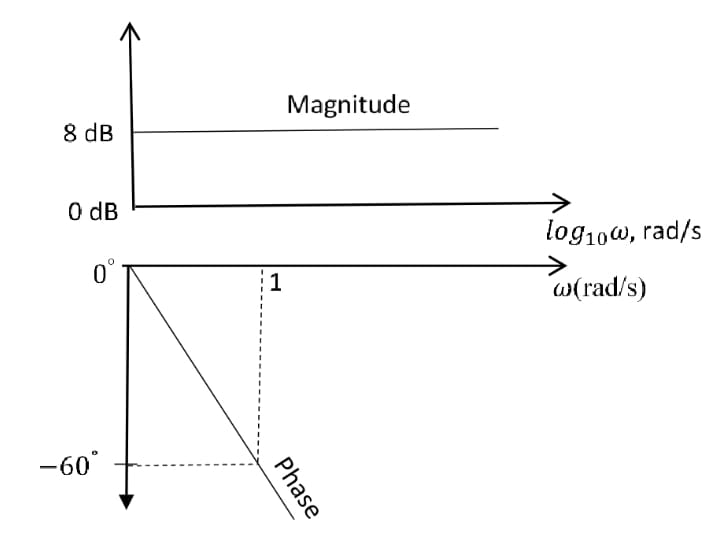
\includegraphics[width=\columnwidth]{figs/gate.jpeg}
        \caption{Graphs}
        \label{fig:1ee36}
    \end{figure}
    \begin{enumerate}
        \item $2.511 e^{-0.0032s}$\\
        \item $\frac{e^{-2.514s}}{s+1}$\\
        \item $1.04e^{-2.514s}$\\
        \item $2.511 e^{-1.047s}$\\
    \end{enumerate}
    
    \solution
    From~\figref{fig:1ee36}
    \begin{align}
        \abs{{H}\brak{j\omega}}&= 8 \\
        \angle H\brak{j\omega} &= \frac{-\pi}{3} \omega
    \end{align}
    Substituting the values from~\figref{fig:1ee36}, magnitude of transfer function is:
    \begin{align}
        8 &= 20\log_{10}(\abs{{H}\brak{j\omega}})\\
        \abs{{H}\brak{j\omega}} &= 10^{0.4} = 2.511
    \end{align}
    Substituting the values from~\figref{fig:1ee36}, The direction of the transfer function is:
    \begin{align}
        \frac{H\brak{j\omega}}{\abs{{H}\brak{j\omega}}} = e^{-j\frac{\pi}{3}\omega}
    \end{align}
    \begin{align}
        H\brak{j\omega} &= 2.511 e^{-j\frac{\pi}{3}\omega} \\
        &= 2.511 e^{-1.047s}
    \end{align}
    \setcounter{figure}{1} % Set figure counter to 1
\end{document}

